\documentclass{beamer}
\usepackage{kotex}
\usepackage{graphicx}
\usepackage{tabularray}
\hypersetup{
	colorlinks = true
}

\title{Pump It Up: 리듬 게임이 아닙니다, 스포츠 게임입니다}
\author{ZeroPage 29기 신연진}

\begin{document}

\frame{\titlepage}

\begin{frame}{목차}
	\tableofcontents
\end{frame}

\begin{frame}{Pump It Up이란?}
	\section{Pump It Up이란?}
	\subsection{Pump It Up 소개}

	\begin{columns}
		\column{0.5\textwidth}
			\includegraphics[width=\columnwidth]{piu-lx.png}	

			\begin{center}
				\small{2017년에 나온 Pump It Up LX 기체, 이 기체가 현재 최신이다.}
			\end{center}
		\column{0.5\textwidth}
		\begin{itemize}
			\item 1999년 8월에 \href{https://www.andamiro.com}{국내기업 안다미로}에서 최초 발매한 리듬게임
			\item 현재 최신버전은 2023년 7월 4일 발매된 Pump It Up PHOENIX 버전.
			\item 발판에서 $ \swarrow, \nwarrow, \square, \nearrow, \searrow $ 총 5개의 화살표를 밟아서 플레이하는 게임이다.
		\end{itemize}	
	\end{columns}
\end{frame}

\begin{frame}{Pump It Up과 DDR의 차이}
	\subsection{Pump It Up과 DDR의 차이}

	\begin{center}
		\begin{tblr}{hlines,vlines}
			\SetRow{azure8,c} & Pump It Up & DDR \\
			사진 & \includegraphics[width=0.3\textwidth]{piu-lx.png} & 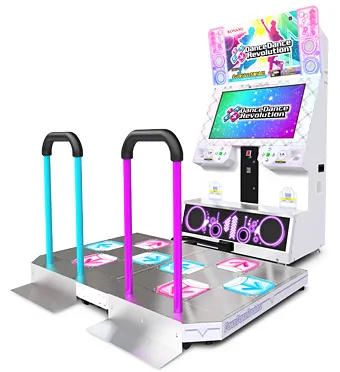
\includegraphics[width=0.3\textwidth]{ddr.png} \\
			발판 & X자형 ($ \swarrow, \nwarrow, \square, \nearrow, \searrow $) & $+$자형 ($ \leftarrow, \rightarrow, \uparrow, \downarrow $) \\
			개발사 & 안다미로 & 코나미 (수입사: 유니아나) \\
			OS & UNIX-Like & Embedded Windows \\
			장르 & 스포츠 & 캐주얼/시물레이션
		\end{tblr}
	\end{center}

	(참고: 장르는 게임물관리위원회 심의결과 기준임)
\end{frame}

\begin{frame}{매너}
	\section{매너}
	\subsection{기본 매너}

	\begin{itemize}
		\item 군화, 구두(특히 하이힐)류를 신고 플레이하지 않는다. (사람이 다치거나 기계가 망가진다.)
		\item 심하게 쾅쾅 밟지 않는다.
		\item 양학하지 않는다.
		\item 기다리는 사람이 있으면 비켜준다.
	\end{itemize}
\end{frame}

\begin{frame}{매너 -- 대기카드(대기코인) 문화}
	\subsection{대기카드(대기코인) 문화}
	
	오락실 위에 카드나 동전, 혹은 지폐가 올려져 있다 $ \rightarrow $ 기다리는 사람이 있다는 뜻
	\begin{itemize}
		\item 이런 경우 자기도 하고 싶으면 상대가 게임을 플레이하고 있지 않을 때(곡을 선곡하고 있을 때) 카드나 동전을 올리면 된다.
		\item 한 사람이 카드나 동전을 2개 이상 올리지 않는다. 비매너임...
		\item 리듬게임 or 마이너한 게임기가 많이 있는 오락실에 있는 문화이고, 그런 오락실이 아니더라도 보통 리듬게임 많이하는 플레이어들은 다 이해한다.
		\begin{itemize}
			\item 근데 인싸들은 이런 문화 당연히 모르니 대충 쓰윽 봐서 알잘딱깔센하게 잘 하면 됨.
		\end{itemize}
	\end{itemize}
\end{frame}

\begin{frame}{AM.PASS}
	\begin{columns}
		\column{0.4\textwidth}
		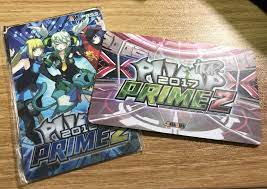
\includegraphics[width=\columnwidth]{am-pass.jpg}

		\column{0.6\textwidth}
		\begin{itemize}
			\item 펌프잇업에서 인터넷에 로그인하는 용도로 쓰는 카드
			\item 오락실에 판매한다. (보통 3,000원에서 5,000원 정도)
			\item 구매한 카드를 \href{https://piugame.com}{공식 홈페이지}에서 등록한 뒤, 카드를 게임기에 찍어 로그인하는 방식
		\end{itemize}
	\end{columns}
\end{frame}

\begin{frame}{게임오버 조건과 팁}
	\begin{itemize}
		\item 51개 이상의 MISS를 연속으로 내면 죽는다. (모드, 스테이지 상관없이 모든 경우에 적용됨)
		\item 상단의 체력 게이지가 떨어지면 죽는다. (단, 베이직 모드, 첫번째 판, (PIU PHOENIX 한정) 프리미엄 모드는 해당되지 않음)
		\item 팁: 롱 노트의 판정은 매우 널널하다.
		\begin{itemize}
			\item 시작 판정이 없다. $ \rightarrow $ 미리 누르고 있어도 PERFECT 판정이 뜬다.
			\item 끝 판정이 없다. $ \rightarrow $ 노트가 끝난 뒤에 발을 떼지 않아도 PERFECT 판정이 뜬다.
			\item 단, 함정카드로 롱 노트위에 바로 일반 노트를 붙이는 경우도 있다.
			\item (예시 영상: \href{https://www.youtube.com/watch?v=720QPEJxJ3o}{채보 수정 업데이트 이전의 Pumptris Quattro S17 플레이 영상})
		\end{itemize}
	\end{itemize}
\end{frame}

\begin{frame}{펌프잇업 용어 -- 무봉}
	\section{펌프잇업 용어}
	\subsection{무봉}

	\begin{columns}
		\column{0.4\textwidth}
		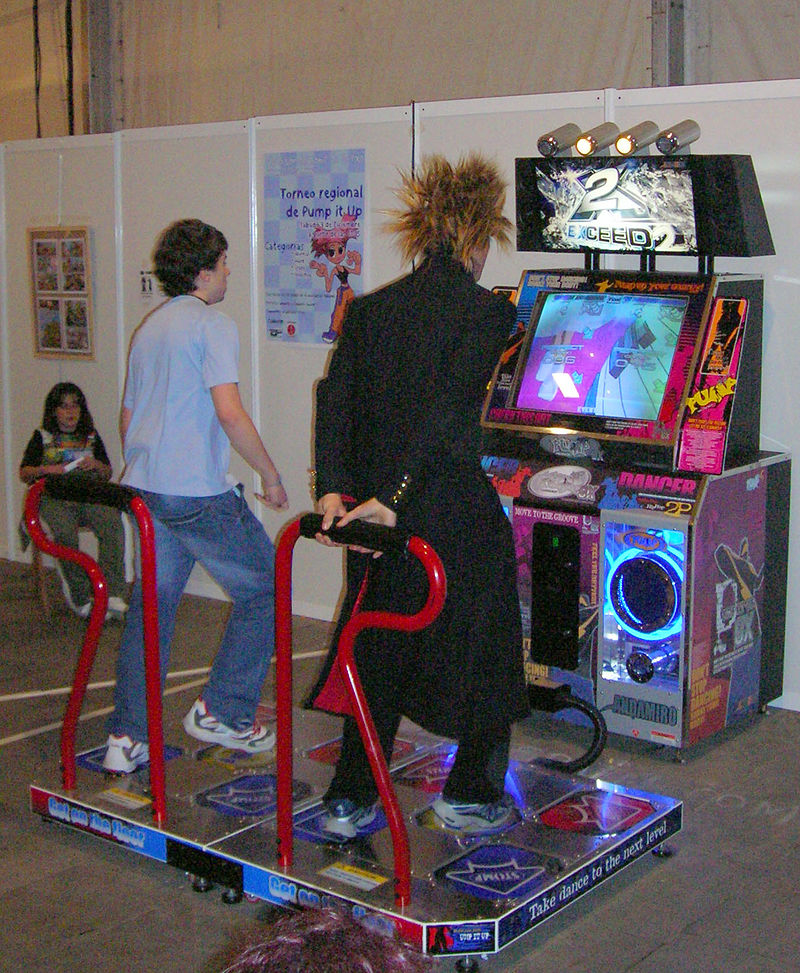
\includegraphics[width=\columnwidth]{piu-bong.jpg}

		\column{0.6\textwidth}
		무봉(or 노봉): 봉을 안 잡고 하는 플레이
		\begin{itemize}
			\item 펌프잇업 발판 뒤에 봉이 있다. 이 봉을 안 잡고 하는 걸 무봉이라 한다. (왼쪽 사진에서 왼쪽 사람이 하는 게 무봉 플레이)
			\item 저난이도대에선 봉 안 잡고도 클리어할 수 있지만, 난이도가 올라갈 수록 어렵기 때문에 그냥 봉 잡고 하는 사람이 더 많다.
		\end{itemize}
	\end{columns}
\end{frame}

\begin{frame}{펌프잇업 용어 -- 싱글, 더블}
	\subsection{싱글, 더블, 코옵, 퍼포먼스}

	\begin{center}
		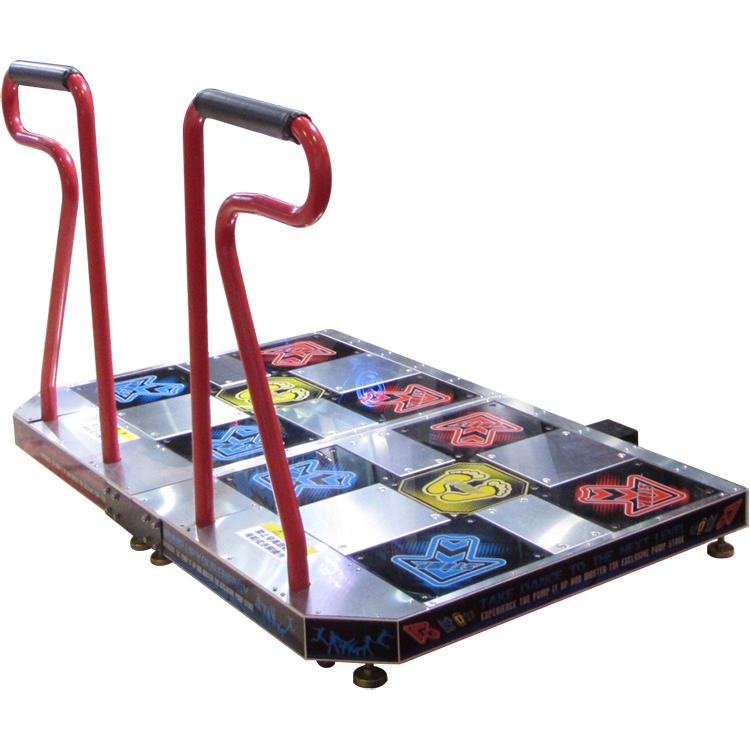
\includegraphics[scale=0.6]{piu-pad.jpg}
	\end{center}
	펌프 발판은 위처럼 생겼다.

	위에서 한 쪽(1P or 2P)만 쓰는 채보는 싱글, 양쪽(1P와 2P 둘다) 다 쓰면 더블 채보.
\end{frame}

\begin{frame}{펌프잇업 용어 -- 코옵}
	\subsection{코옵, 퍼포먼스}
	\begin{itemize}
		\item 코옵 \\ 2명 이상의 사람이 동시에 하는 더블채보 \\ 1P, 2P, 3P, 4P, ..., nP가 밟는 화살표가 구분되어 있다. \\ (참고영상: \href{https://www.youtube.com/watch?v=hr1w7kXJqgA}{BOSS\_PIUVN의 Tribe Attacker CO-OP X4 풀레이 영상})
		\item 퍼포먼스 \\ 어그로 \\ (참고 영상: \href{https://www.youtube.com/watch?v=PqCh-_Tvbf8}{Pump it up WPF 2016에서의 일본팀 퍼포먼스 플레이 영상})
	\end{itemize}
\end{frame}

% 겹발
% 틀기, 끌기, 비비기, 떨기, 하프, 체동
% 브렉 온, 브렉오프, 51미스
% 베이직, 풀, 하트시스템, 커맨드

\begin{frame}{플레이 스킬 -- 틀기, 끌기, 떨기, 비비기}
	\section{플레이 스킬}
	\subsection{틀기, 끌기, 떨기, 비비기}
	\begin{itemize}
		\item 특정 레벨대 이후부터 \textbf{틀기}를 해야하는 패턴이 나온다. 틀기란
		      패턴을 왼발, 오른발을 번걸아가며 밟는 것을 의미한다. (번갈아가며 밟다보면 허리가 자동으로 틀어져서 ``틀기''라고 함.) \\
			  (관련 영상 \#1: \href{https://www.youtube.com/watch?v=VO0ecPF6TEs}{REICON의 Canon D S10 플레이 영상}) \\
			  (관련 영상 \#2: \href{https://www.youtube.com/watch?v=seMfO-xS3GI}{REICON의 Pump Me Amadeus S11 플레이 영상})
		\item 모두 다 틀기만 하면 힘든 패턴 or 체력이 떨어졌을 때는 \textbf{끌기}를 할 수도 있다. 끌기는 먼저 밟은 발로 다른 스텝을 밟는 것을 의미한다.
		\item 두 발로 두 화살표를 번갈아가며 밟는 패턴도 있다. 이건 \textbf{떨기}라고 한다. \\
		(참고자료: \href{https://www.youtube.com/shorts/KMKJqTbQ-nQ}{JIWOOKIM의 떨기 영상})
		\item 비비기: 운에 모든 걸 걸고 일단 보이는대로 막 밟는 것...
	\end{itemize}
\end{frame}

\begin{frame}{플레이 스킬 -- 하프}
	\section{하프}
	\begin{center}
		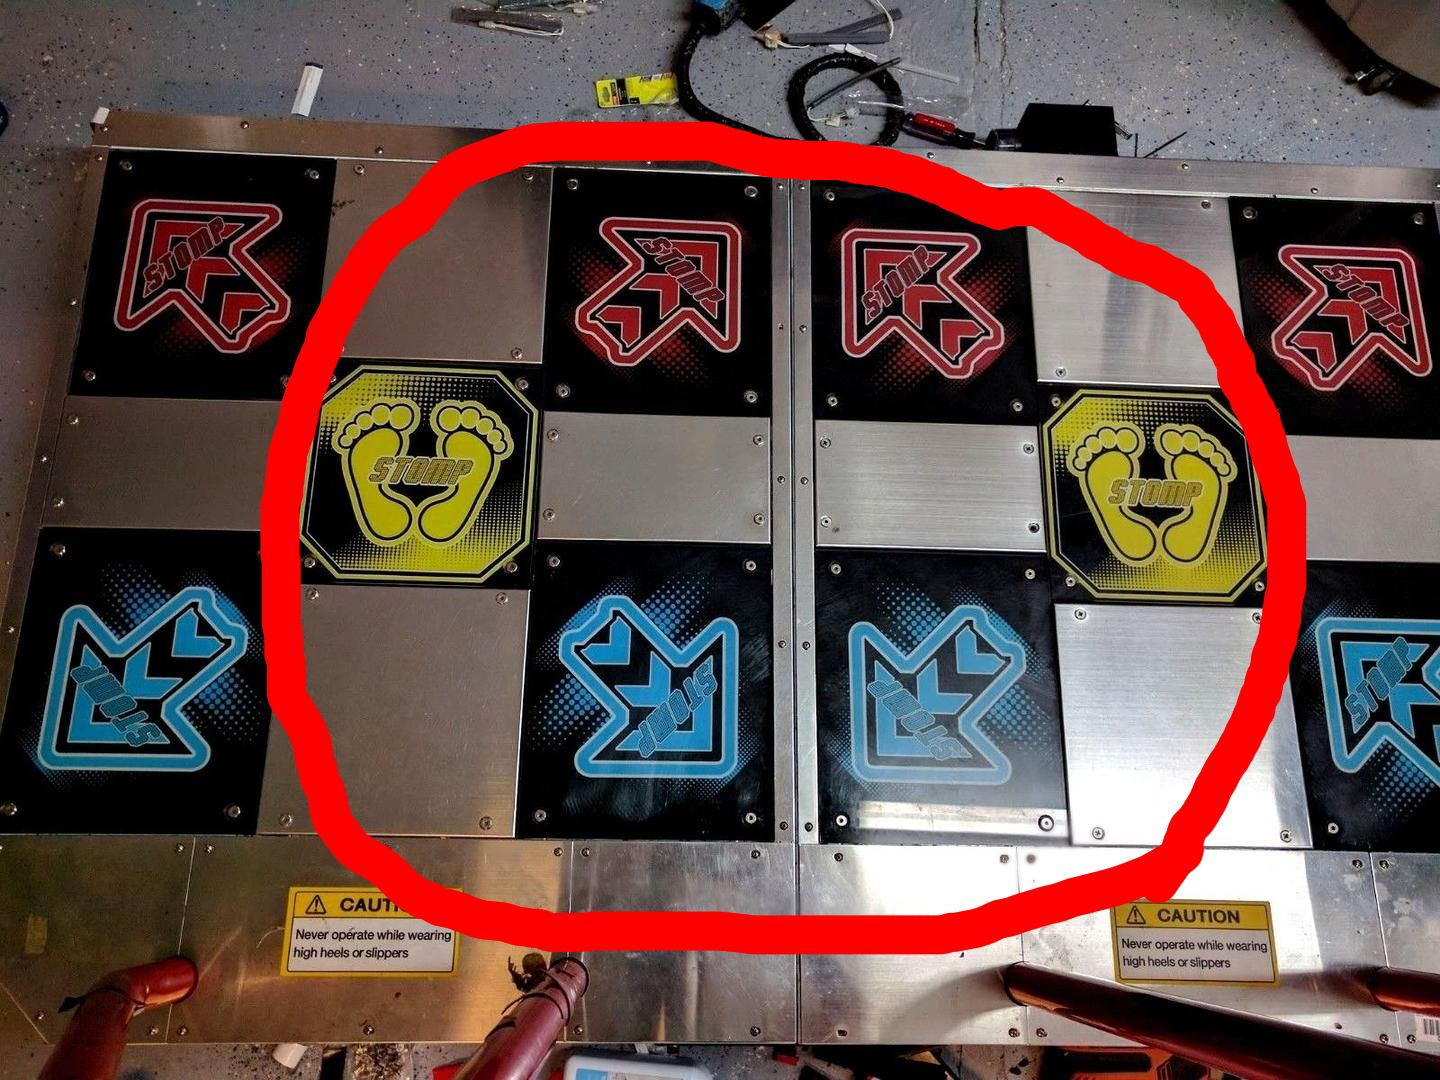
\includegraphics[scale=0.135]{piu-half.jpg}
	\end{center}

	하프: 더블채보에서 중간부분 (사진에서 동그라미친 부분)을 의미한다. \\
	(관련 영상 \#1: \href{https://www.youtube.com/watch?v=emOEtjVNjqw}{Super Fantasy D18}) \\
	(관련 연상 \#2: \href{https://www.youtube.com/watch?v=gdDAkSXkn9k}{잡동사니 이노센스 D16})
\end{frame}

\begin{frame}
	\begin{center}
		감사합니다!
	\end{center}
\end{frame}

\end{document}
